\documentclass[letterpaper,12pt,notitlepage,twoside]{report}

%\newcommand{\watermark}{Deep Learning}
\newcommand{\booktopic}{Deep Learning}
\newcommand{\lastname}{Okoli}
\usepackage{NoteStyle}
\usepackage{placeins}
\usepackage{enumitem}
\usepackage{listings}

\definecolor{codegreen}{rgb}{0,0.6,0}
\definecolor{codegray}{rgb}{0.5,0.5,0.5}
\definecolor{codepurple}{rgb}{0.58,0,0.82}
\definecolor{backcolour}{rgb}{0.95,0.95,0.92}

\lstdefinestyle{mystyle}{
    backgroundcolor=\color{backcolour},   
    commentstyle=\color{codegreen},
    keywordstyle=\color{magenta},
    numberstyle=\tiny\color{codegray},
    stringstyle=\color{codepurple},
    basicstyle=\ttfamily\footnotesize,
    breakatwhitespace=false,         
    breaklines=true,                 
    captionpos=b,                    
    keepspaces=true,                 
    numbers=left,                    
    numbersep=5pt,                  
    showspaces=false,                
    showstringspaces=false,
    showtabs=false,                  
    tabsize=2
}

\lstset{style=mystyle}

\title{Deep Learning}
\author{Chuks Okoli}
\date{\footnotesize Last Updated: \today}

\hypersetup{
  pdftitle={Deep Learning},
  pdfauthor={Chuks Okoli},
  pdfsubject={},
}


% ToC on the title page:
% https://tex.stackexchange.com/a/45863
\makeatletter
\newcommand*{\toccontents}{\@starttoc{toc}}
\makeatother

\begin{document}

\begin{titlepage}
  \pagestyle{plain}
  \maketitle
  \setcounter{tocdepth}{2}

  \pdfbookmark[section]{\contentsname}{toc}
  \toccontents
  % Separate page:
  % \tableofcontents
\end{titlepage}

\chapter{Welcome to Deep Learning} \label{ch:1}
\inspiration{Just as electricity transformed almost everything 100 years ago, today I actually have a hard time thinking of an industry that I don’t think AI (Artificial Intelligence) will transform in the next several years.}{Andrew Ng}{DeepLearning.AI}

\firstletter{Hello there}, and welcome to \booktopic. This work is a culmination of hours of effort to create my reference for deep learning. All the explanations are in my own words but majority of the contents are based on DeepLearning.AI's specialization in \href{https://www.deeplearning.ai/courses/deep-learning-specialization/}{Deep Learning}.


\section{Introduction to Deep learning}
The term, Deep Learning, refers to training Neural Networks, sometimes very large Neural Networks.  In order to predict the price of a house based on its size for example, we can apply linear regression as a method for fitting a function to predict house prices. An alternative approach would be to use a simple neural network to model the relationship between house size and price. 

The simple neural network consists of a single neurons, which takes an input (e.g., house size) and outputs a prediction (e.g., house price). The neuron computes a linear function of the input and applies a rectified linear unit (ReLU) activation function to ensure non-negativity. Each neuron in the network computes a function of the input features and contributes to the overall prediction. When extended to multiple features, each feature is represented by a separate neuron, and the network learns to predict the house price based on these features.

Neural networks are useful in supervised learning scenarios, where the goal is to map input features to corresponding output labels. Given enough training data, neural networks can learn complex mappings from inputs to outputs.

\begin{figure}[h]
	\centering
	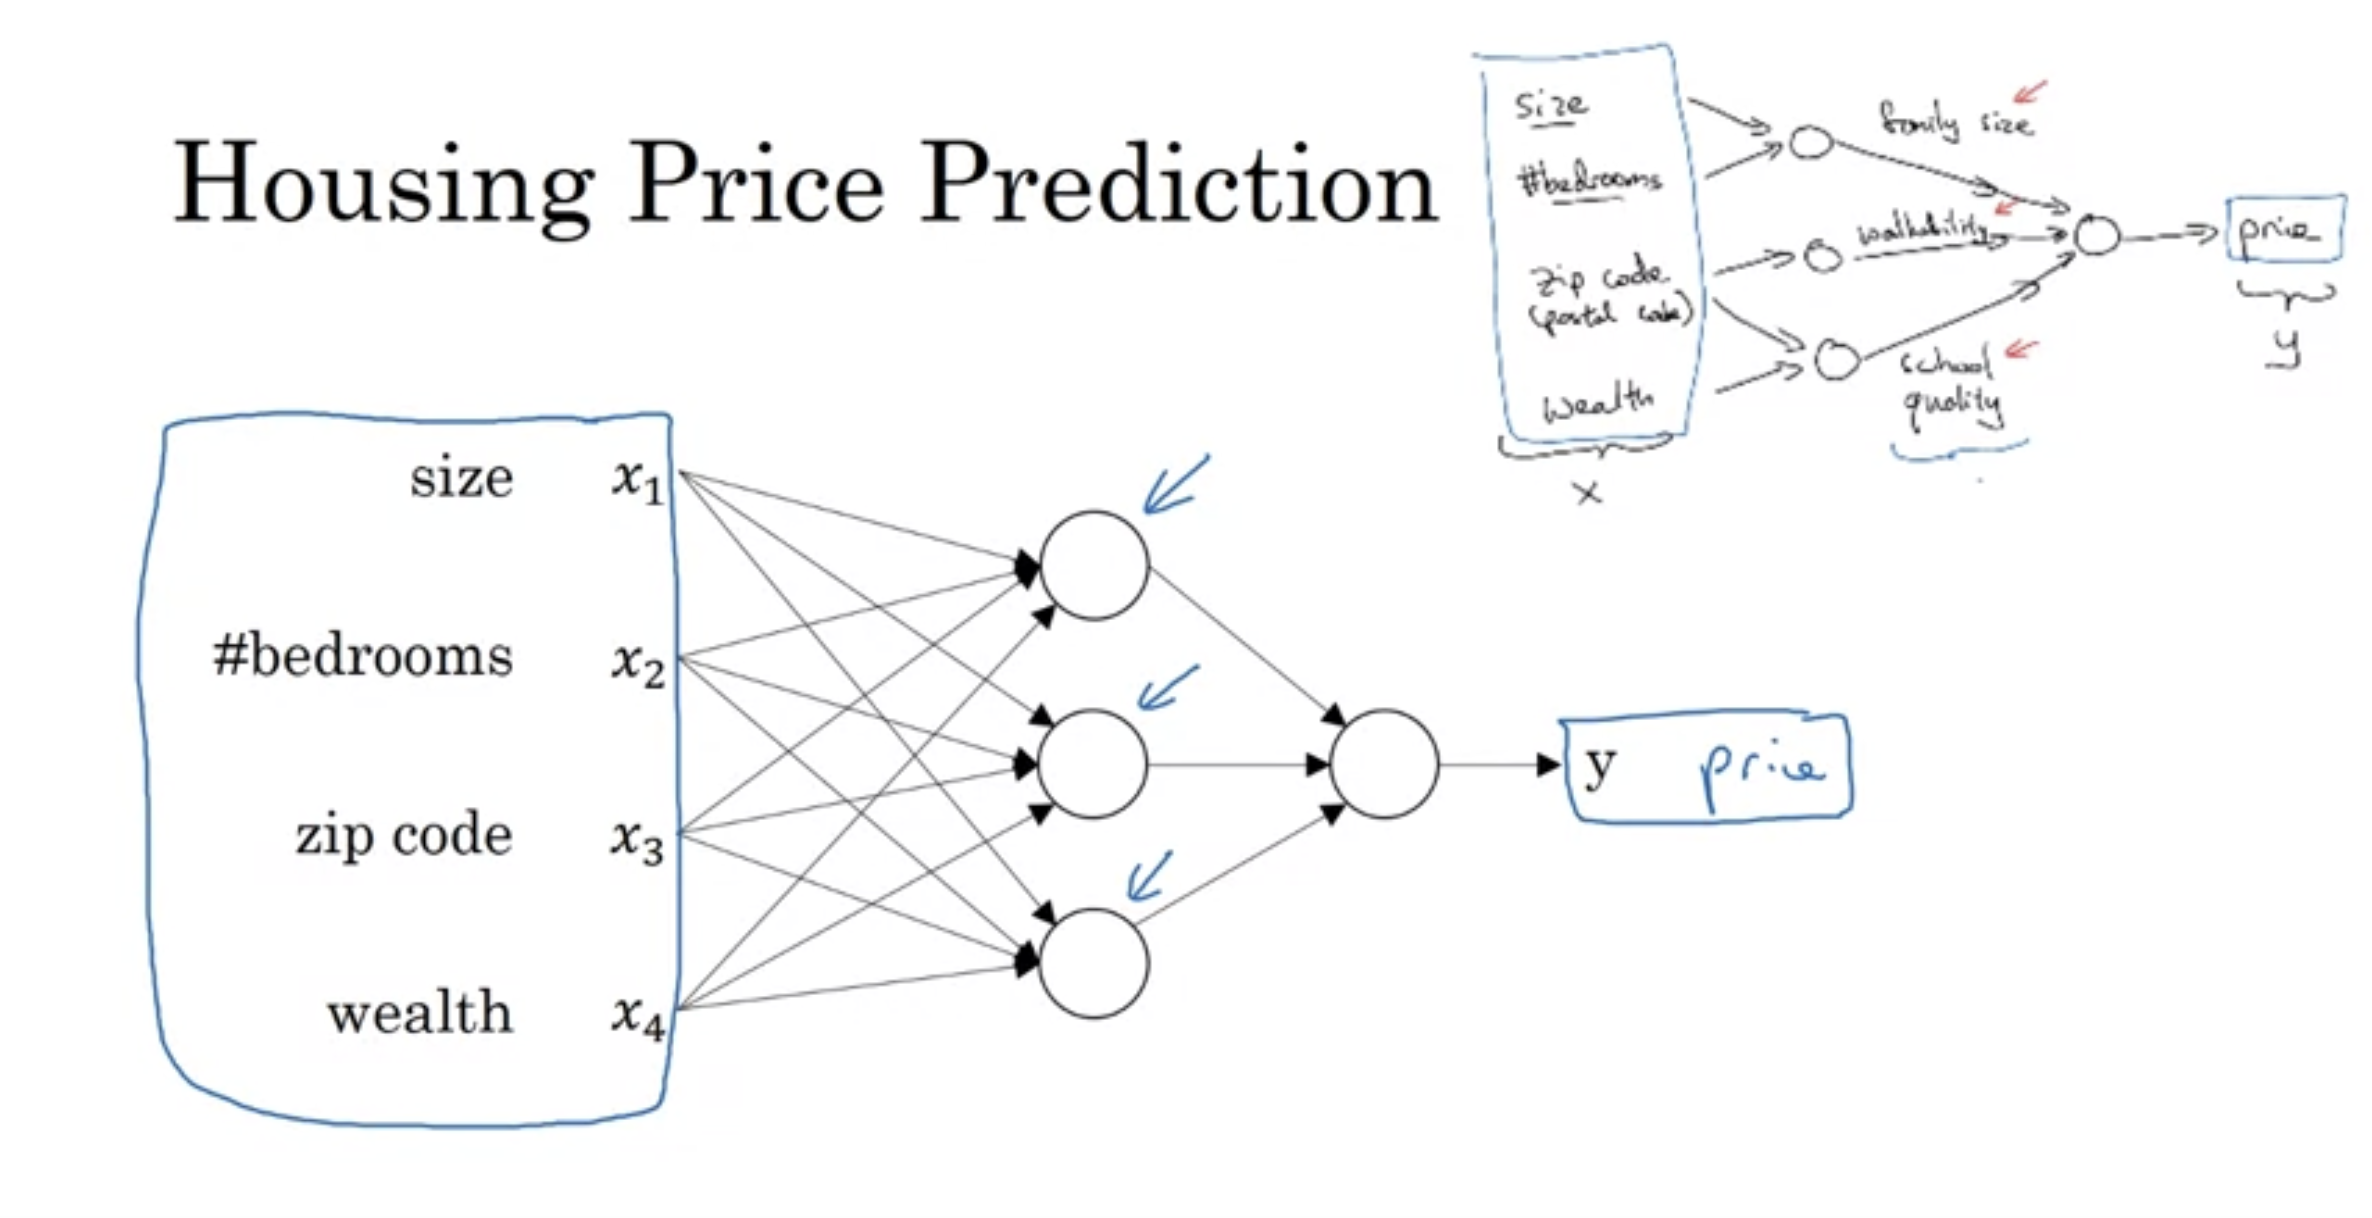
\includegraphics[width=0.75\textwidth]{Images/Simple Neural Network.png}
	\caption{A Simple Neural Network for House Price Prediction}
	\label{fig:1}
\end{figure}
\FloatBarrier

\subsection{Supervised Learning with Neural Networks}
Neural networks have gained a lot of attention lately for their ability to solve complex problems effectively. In supervised learning, you input data and aim to predict an output. Examples include predicting house prices or online ad clicks. Neural networks have been successful in various applications, like online advertising, computer vision, speech recognition, and machine translation. Different types of neural networks are used based on the nature of the data, such as convolutional neural networks for images and recurrent neural networks for sequential data. Structured data, like database entries, and unstructured data, like images or text, are both now interpretable by neural networks, thanks to recent advancements. While neural networks are often associated with recognizing images or text, they also excel in processing structured data, leading to improved advertising and recommendation systems. The techniques covered in this course apply to both structured and unstructured data, reflecting the versatility of neural networks in various applications.

\begin{figure}[h]
	\centering
	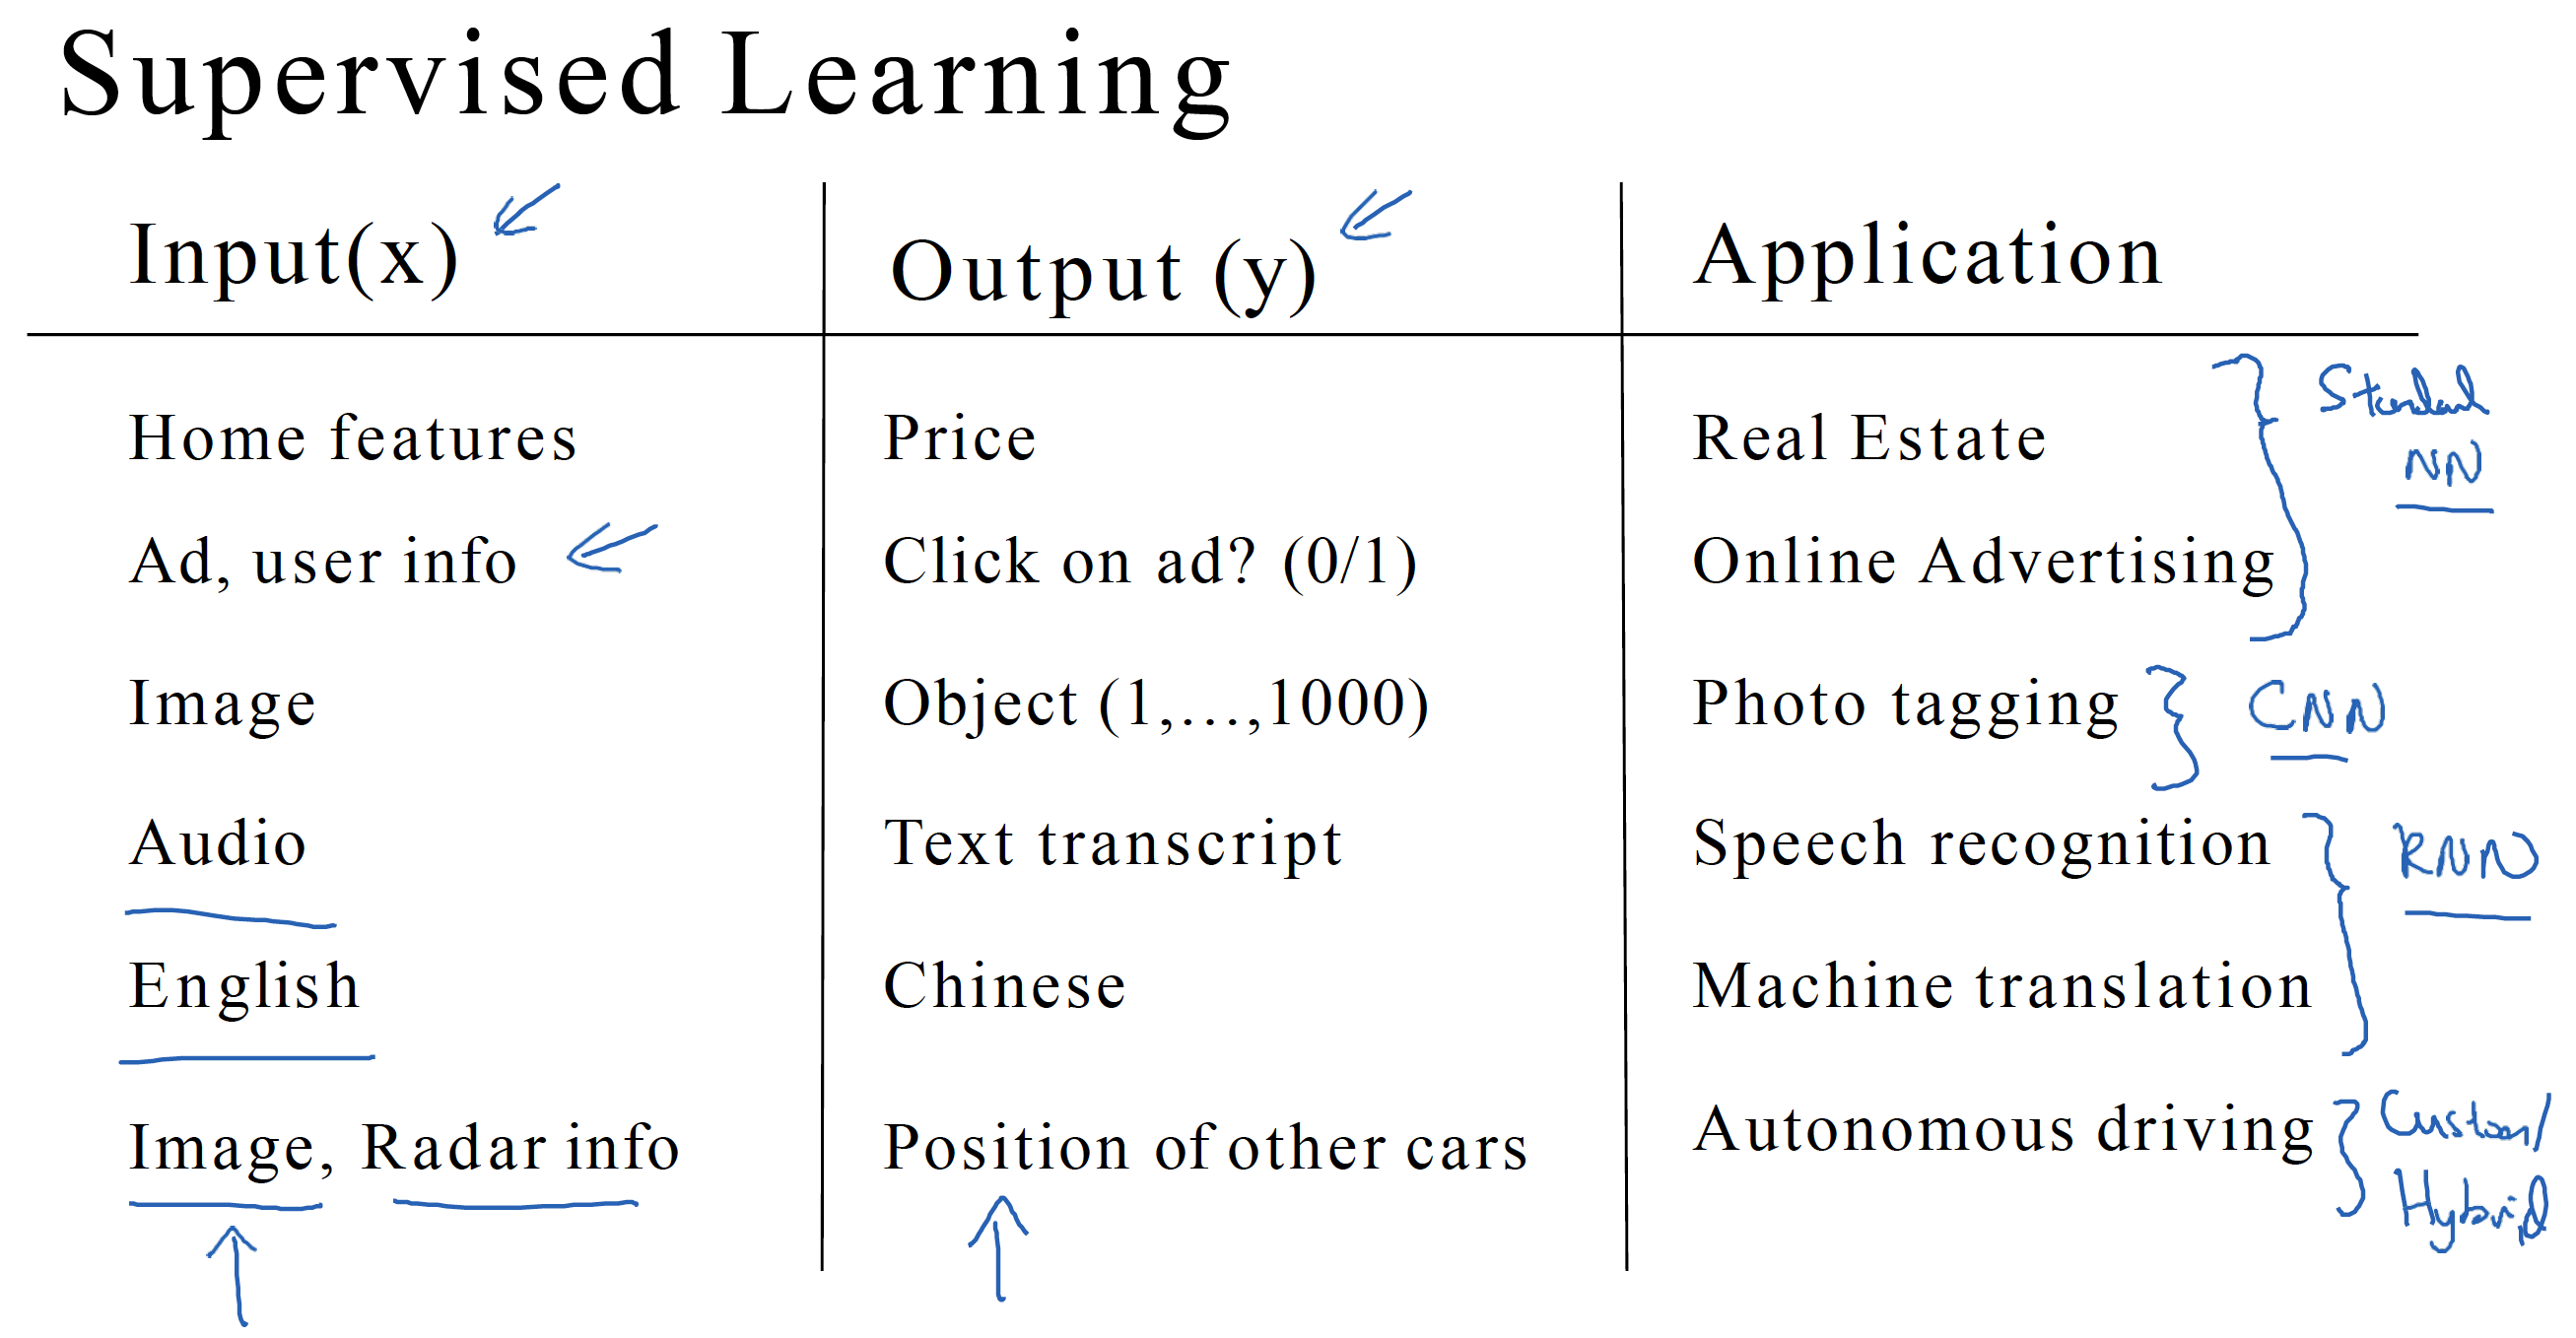
\includegraphics[width=0.75\textwidth]{Images/Supervised learning.png}
	\caption{Examples of Supervised learning}
	\label{fig:2}
\end{figure}

\begin{figure}[h]
	\centering
	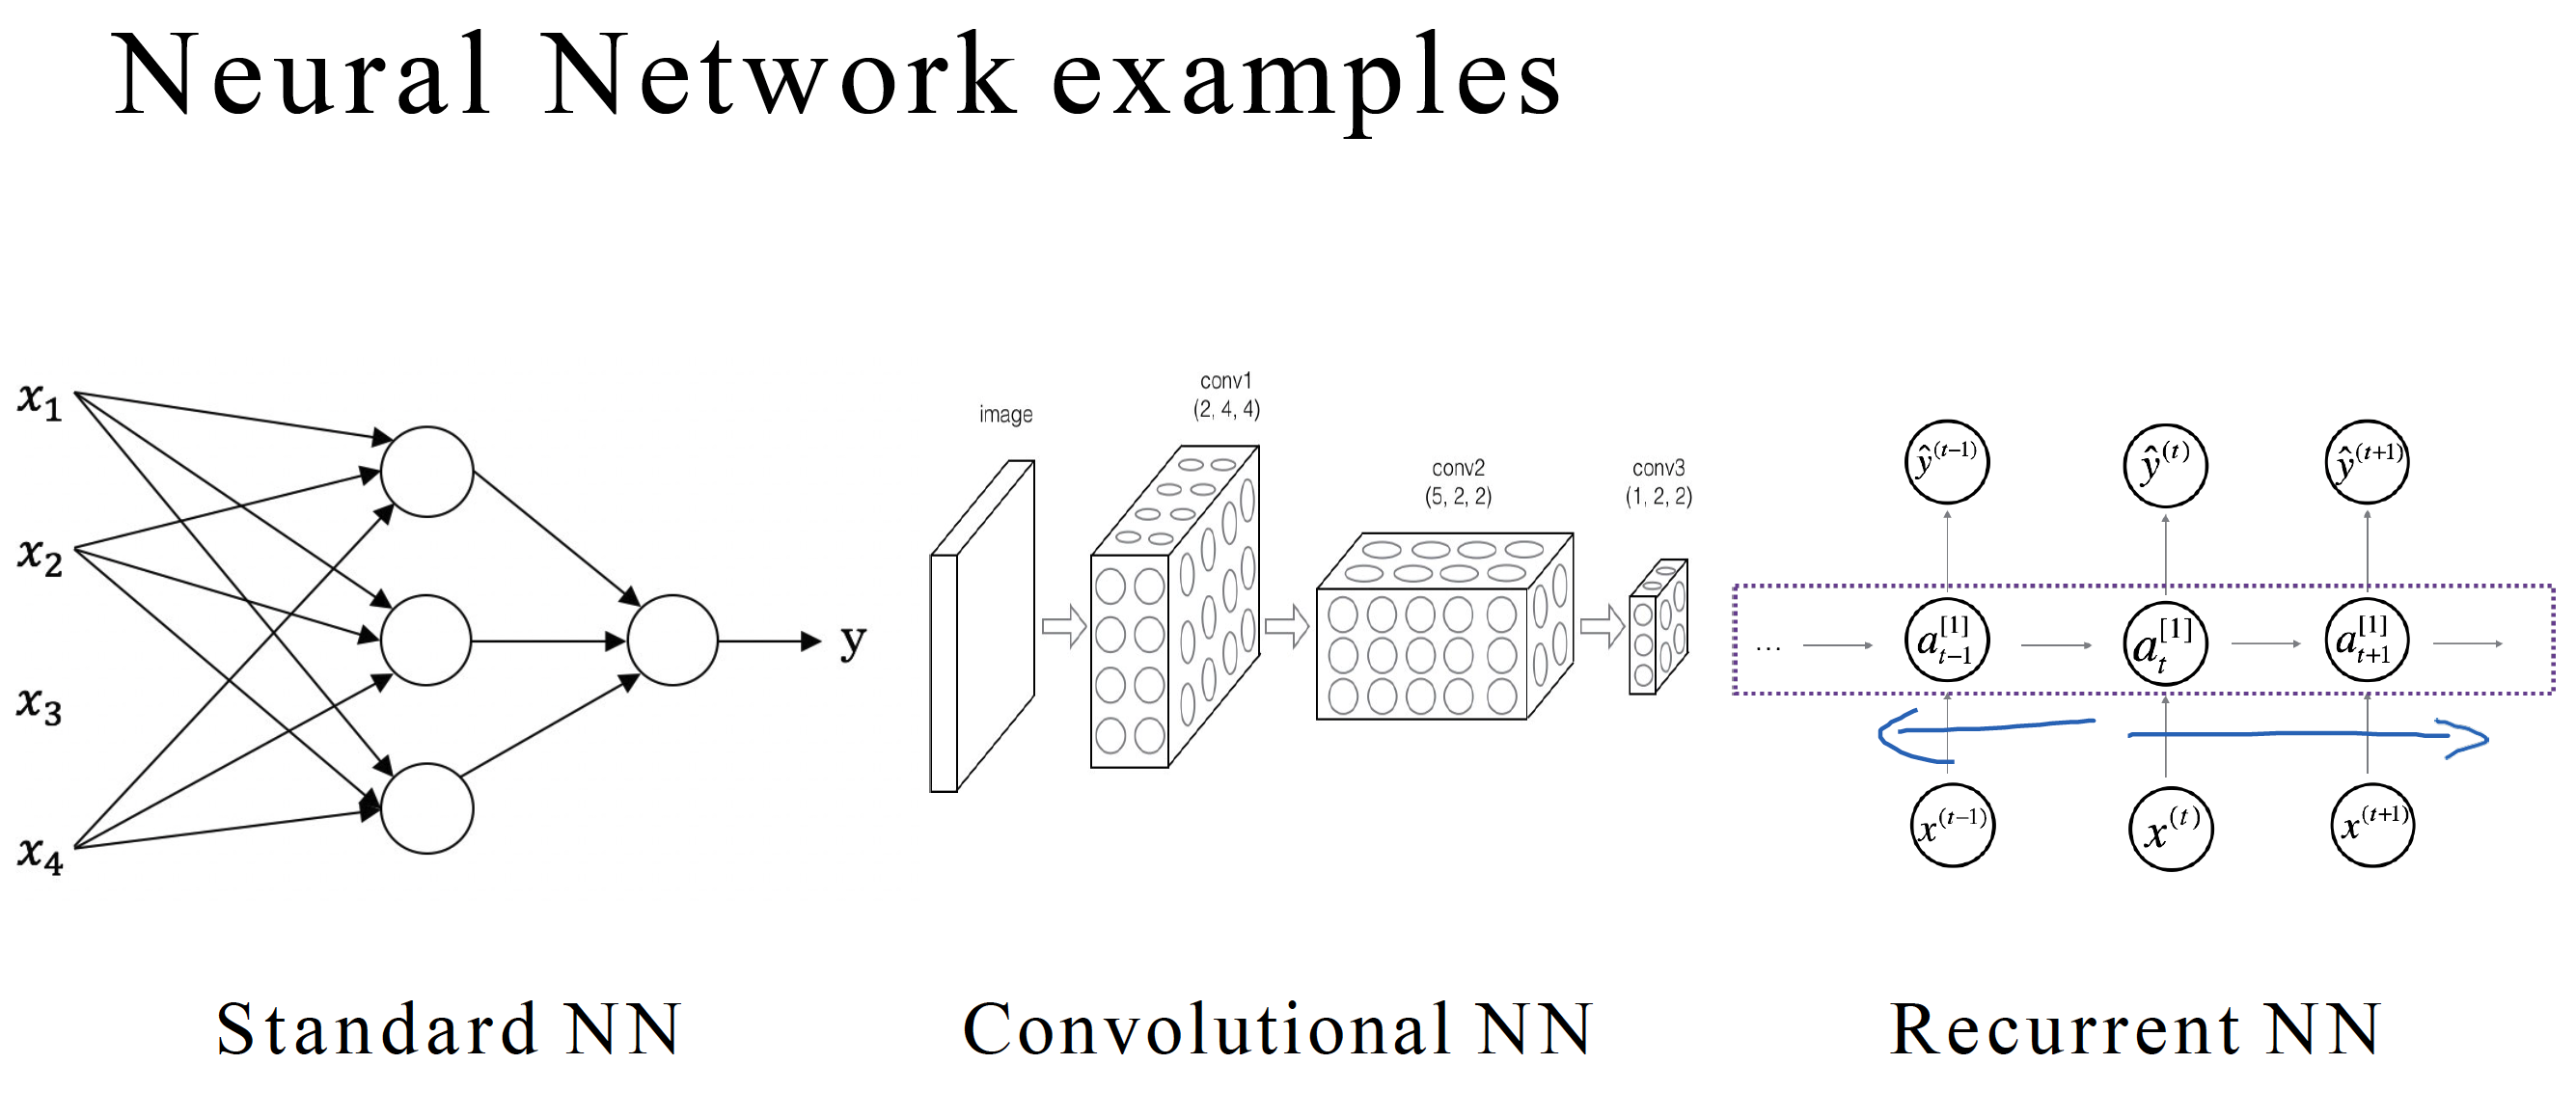
\includegraphics[width=0.75\textwidth]{Images/Neural network examples.png}
	\caption{Neural network examples}
	\label{fig:3}
\end{figure}
\FloatBarrier

\subsection{Why is Deep Learning taking off?}
The rise of deep learning has been fueled by several key factors. One major driver is the abundance of data available for training machine learning models. With the digitization of society, activities performed on digital devices generate vast amounts of data, enabling neural networks to learn from large datasets. Additionally, advancements in hardware, such as GPUs and specialized processors, have facilitated the training of large neural networks by providing faster computation speeds. Algorithmic innovations, like the adoption of the ReLU activation function, have also played a crucial role in accelerating learning processes. By reducing the time required to train models and enabling faster experimentation, these innovations have enhanced productivity and fostered rapid progress in deep learning research. Moving forward, the continued growth of digital data, advancements in hardware technology, and ongoing algorithmic research are expected to further drive improvements in deep learning capabilities. As a result, deep learning is poised to continue evolving and delivering advancements in various applications for years to come.

\begin{funfact}[frametitle=\facttitlep{FunFact}{What's drives Deep Learning}]
Deep Learning took off in the last few years and not before mainly because of great computing power and huge amount of data. These two are the key components for the successes of deep learning. The performance of a neural network improves with more training data.
\end{funfact}

\begin{figure}[h]
	\centering
	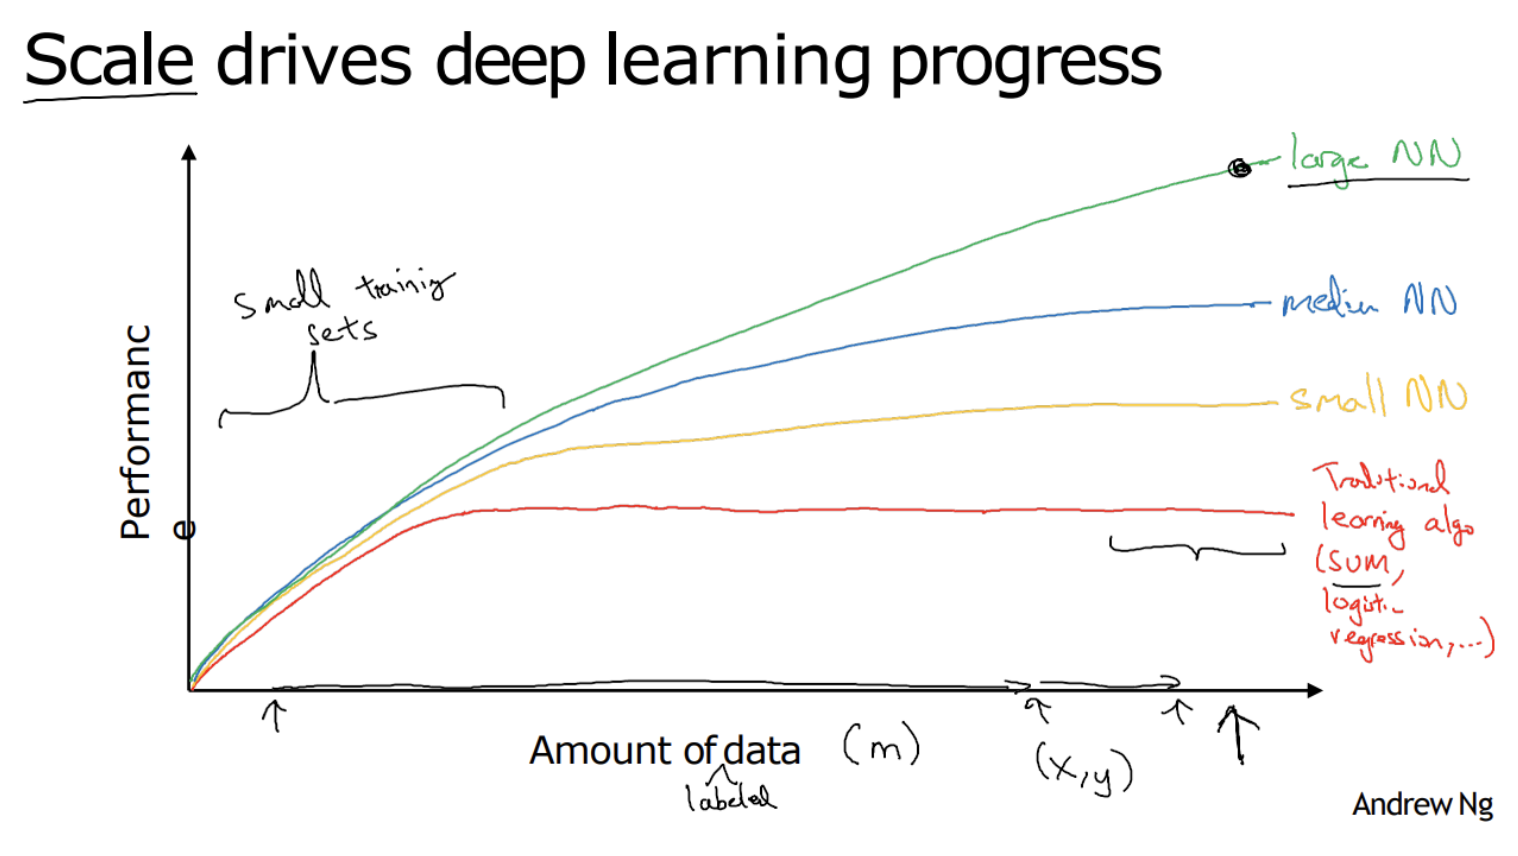
\includegraphics[width=0.75\textwidth]{Images/Scale and neural network.png}
	\caption{Scale drives neural networks}
	\label{fig:4}
\end{figure}
\FloatBarrier

\section{Neural Network Basics}
\subsection{Logistic Regression as a Neural Network}
Logistic regression is an algorithm for binary classification problem.  In a binary classification problem,  the goal is to train a classifier for which the input is an image represented by a feature vector, $x$, and predicts whether the corresponding label $y$ is 1 or 0. In this case, whether this is a cat image (1) or a non-cat image (0). 

\begin{figure}[h]
	\centering
	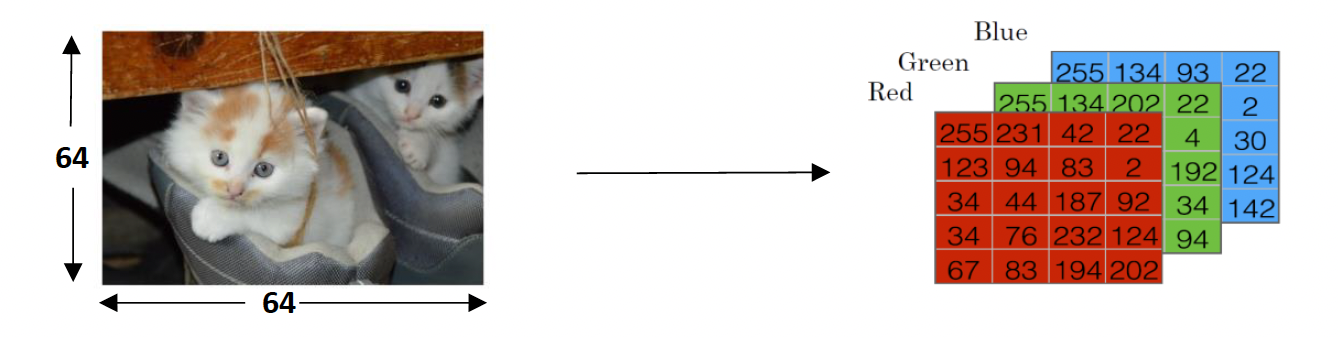
\includegraphics[width=0.95\textwidth]{Images/Binary classification cat example.png}
	\caption{Binary classification - Cat vs Non-Cat}
	\label{fig:5}
\end{figure}
\FloatBarrier

An image is stored in the computer in three separate matrices corresponding to the Red, Green, and Blue color channels of the image. The three matrices have the same size as the image, for example, the resolution of the cat image is 64 pixels x 64 pixels, the three matrices (RGB) are 64 x 64 each. The value in a cell represents the pixel intensity which will be used to create a feature vector of $n$ dimension. In pattern recognition and machine learning, a feature vector represents an image, Then the classifier's job is to determine whether it contain a picture of a cat or not.
To create a feature vector, $x$, the pixel intensity values will be ``unrolled'' or ``reshaped'' for each color. The dimension of the input feature vector $x$ is $n = 64* 64* 3 = 12288$. Hence, we use $n_x = 12288$ to represent the dimensions of the feature vectors. 

\begin{figure}[h]
	\centering
	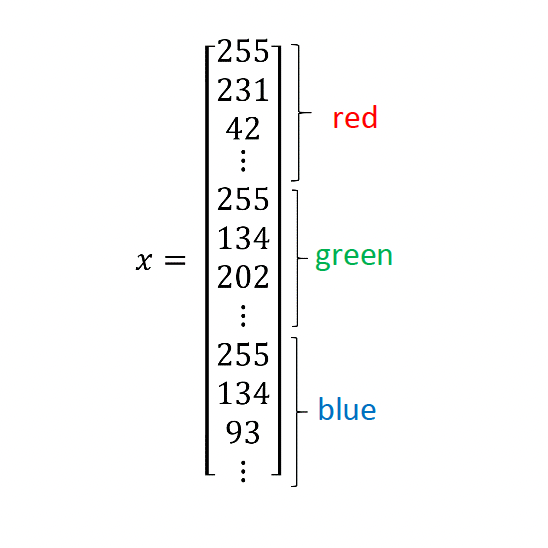
\includegraphics[width=0.35\textwidth]{Images/Reshaped feature vector.png}
	\caption{Reshaped feature vector}
	\label{fig:6}
\end{figure}
\FloatBarrier

\subsubsection{Logistic Regression}
In Logistic regression, the goal is to minimize the error between the prediction and the training data. Given an image represented by a feature vector $x$, the algorithm will evaluate the probability of a cat being in that image.

\begin{equation}
\text{Given}~ x , \hat{y} = P(y=1|x), \text{where}~0 \leq \hat{y} \leq 1
\end{equation}
The parameters used in Logistic regression are:
\begin{itemize}
\item The input features vector: $x \in \mathbb{R}^{n_x}$, where $n_x$ is the number of features
\item The training label: $y \in 0,1$
\item The weights: $w \in \mathbb{R}^{n_x}$, where $n_x$ is the number of features
\item The threshold: $b \in \mathbb{R}$
\item The output: $\hat{y} = \sigma*(w^T*x+b)$
\item Sigmoid function: $s = \sigma(w^T*x+b) = \sigma(z)= \frac{1}{1+e^{-z}}$
\end{itemize}
$w^T*x+b$ is a linear function $(ax+b)$, but since we are looking for a probability constraint between $[0,1]$, the sigmoid function is used. The function is bounded between $[0,1]$ as shown in the graph above.
Some observations from the graph:
\begin{itemize}
\item If $z$ is a large positive number, then $\sigma(z) = 1$
\item If $z$ is small or large negative number, then $\sigma(z) = 0$
\item If $z=0$, then $\sigma(z) = 0.5$
\end{itemize}





%
\begin{itemize}
  \item Like this one,
    \begin{notebox}
      which is wrapped in gray. I use it for notes.\ldots
    \end{notebox}

  \item Or this one,
    \begin{funfact}
      which is wrapped in red. I use it for fun facts or other asides\ldots
    \end{funfact}

  \item Or this one,
    \begin{mathaside}
      which is wrapped in blue and used for mathy stuff.
    \end{mathaside}

  \item Or this last one,
    \begin{example}
      which is wrapped in green. With a title, it's used for enumerated examples
      (see \smtt{\textbackslash extitle} and \smtt{\textbackslash excounter}).
      Observe:
    \end{example}

    \begin{example}[frametitle=\extitle{Test}]
      This is an example. What's the answer to $2+2$?
      \answer{Obviously 4, lol.}
    \end{example}

    \begin{example}[frametitle=\extitle{Test Again}]
      This one will increment the counter automatically, resetting for each
      chapter.
    \end{example}


  \item For red and blue boxes, there are custom commands for titles, too:
    \begin{mathaside}[frametitle=\mathtitle{One Title}]
      Like this
    \end{mathaside}
    \begin{mathaside}[frametitle=\mathtitlep{Two Titles}{A Subtitle}]
      Or this
    \end{mathaside}
\end{itemize}

\hr{5in}

These styles also automatically apply to theorems and claims.

\begin{theorem}[Pythagorean Theorem]
  \label{thm:pyth}
  For any right triangle with legs $a,b$ and hypotenuse $c$:
  %
  \begin{equation}
    \label{eq:pyth}
    a^2+b^2=c^2
  \end{equation}
\end{theorem}
\begin{proof}
  This is left as an exercise to the reader.
\end{proof}

\begin{claim}
  This is the greatest note template in the world.
\end{claim}

\hr{5in}

There are different ways to quote things, too, depending on how you want to
emphasize:

\begin{quoting}
  This is a simple, indented quote with small letters and italics usually
  suitable for in-text quotations when you just want a block.
\end{quoting}

Alternatively, you can use the \smtt{\textbackslash inspiration} command from
the chapter heading, which leverages the \smtt{thickleftborder} frame
internally, but adds a little more padding and styling (there's also just
\smtt{leftborder} for a thinner variant):

\begin{thickleftborder}
  Hello there!
\end{thickleftborder}



\section{On Cross-Referencing}
\marginnote{\footnotesize\softtext This is the standard way to include margin
notes. There are also commands to link to source papers directly (see
\smtt{\textbackslash lesson}).} You can reference most things---see
\autoref{thm:pyth} or \eqref{eq:pyth} or the \nameref{ch:1} chapter---directly
and easily as long as you give them labels. These are ``built-ins.'' However,
you can also create a \term{custom term} that will be included in the index,
then include references to it that link back to the original definition. Try
clicking: \refterm{custom term}. Building the index is on you, though. You can
also reference by using a different term for the text: \reftermx{custom
term}{like this}. Sometimes it doesn't fit the \termx{grammar}{grammatical
structure} of the sentence so you can define the term one way and visualize it
another way (this creates a \aterm{grammar} entry in the index). There's also
\prop{math terms} and a way to reference them: \refprop{math terms} (clickable),
but they do \textbf{not} show up in the index.



\section{On Math}
Most of the math stuff is just macros for specific things like the convolution
operator, $\conv$, probabilities, $\cprob{A}{B=C}$, or big-$O$ notation,
$\bigO{n^2\log{n}}$ but there's also a convenient way to include explanations on
the side of an equation:
%
\begin{align*}
  1 + 1 &\overset{?}{=} 2    \sideblock{2in}{first we do this} \\
      2 &\overset{?}{=} 2    \sideblock{2in}{then we do this} \\
      2 &= 2 \qed
\end{align*}

These are all in the \smtt{CustomCommands.sty} file.



\end{document}

